%Tipo de Documento [Conferencia]

\documentclass[conference]{IEEEtran}\usepackage[]{graphicx}\usepackage[]{color}
%% maxwidth is the original width if it is less than linewidth
%% otherwise use linewidth (to make sure the graphics do not exceed the margin)
\makeatletter
\def\maxwidth{ %
  \ifdim\Gin@nat@width>\linewidth
    \linewidth
  \else
    \Gin@nat@width
  \fi
}
\makeatother

\definecolor{fgcolor}{rgb}{0.345, 0.345, 0.345}
\newcommand{\hlnum}[1]{\textcolor[rgb]{0.686,0.059,0.569}{#1}}%
\newcommand{\hlstr}[1]{\textcolor[rgb]{0.192,0.494,0.8}{#1}}%
\newcommand{\hlcom}[1]{\textcolor[rgb]{0.678,0.584,0.686}{\textit{#1}}}%
\newcommand{\hlopt}[1]{\textcolor[rgb]{0,0,0}{#1}}%
\newcommand{\hlstd}[1]{\textcolor[rgb]{0.345,0.345,0.345}{#1}}%
\newcommand{\hlkwa}[1]{\textcolor[rgb]{0.161,0.373,0.58}{\textbf{#1}}}%
\newcommand{\hlkwb}[1]{\textcolor[rgb]{0.69,0.353,0.396}{#1}}%
\newcommand{\hlkwc}[1]{\textcolor[rgb]{0.333,0.667,0.333}{#1}}%
\newcommand{\hlkwd}[1]{\textcolor[rgb]{0.737,0.353,0.396}{\textbf{#1}}}%

\usepackage{framed}
\makeatletter
\newenvironment{kframe}{%
 \def\at@end@of@kframe{}%
 \ifinner\ifhmode%
  \def\at@end@of@kframe{\end{minipage}}%
  \begin{minipage}{\columnwidth}%
 \fi\fi%
 \def\FrameCommand##1{\hskip\@totalleftmargin \hskip-\fboxsep
 \colorbox{shadecolor}{##1}\hskip-\fboxsep
     % There is no \\@totalrightmargin, so:
     \hskip-\linewidth \hskip-\@totalleftmargin \hskip\columnwidth}%
 \MakeFramed {\advance\hsize-\width
   \@totalleftmargin\z@ \linewidth\hsize
   \@setminipage}}%
 {\par\unskip\endMakeFramed%
 \at@end@of@kframe}
\makeatother

\definecolor{shadecolor}{rgb}{.97, .97, .97}
\definecolor{messagecolor}{rgb}{0, 0, 0}
\definecolor{warningcolor}{rgb}{1, 0, 1}
\definecolor{errorcolor}{rgb}{1, 0, 0}
\newenvironment{knitrout}{}{} % an empty environment to be redefined in TeX

\usepackage{alltt}

%BIBLIOTECAS

% Este paquete se utiliza para generar texto o graficas de relleno.
%\usepackage{blindtext, graphicx}
%Biblioteca para graficas
\usepackage{graphicx}
%Biblioteca para lectura de caracteres ortográficos (tildes..etc. ) 
\usepackage[utf8]{inputenc}
%Biblioteca para enumeración de imagenes
\usepackage{float}
%Biblioteca para graficos vectrizados.svg 
\usepackage{svg}
\usepackage{enumerate}
%Biblioteca para enumerar figuras tablas.. etc en español 
\usepackage[spanish, es-tabla]{babel}
\usepackage[spanish]{babel}
%\usepackage[spanish,USenglish]{babel}

%INICIO DEL DOCUMENTO
\IfFileExists{upquote.sty}{\usepackage{upquote}}{}
\begin{document}
	
	
	% TITULO DEL PAPER
\title{Modelo predictivo para estimar el crecimiento poblacional hispano al a\~no 2020 en diferentes ciudades de EEUU}

% NOMBRE DE LOS AUTORES
\author{
	\IEEEauthorblockN{Leonel Muñoz Cedano}
	\IEEEauthorblockA{Ingeniero de Sistemas\\ 
		Universidad Distrital Francisco José de Caldas\\
		Bogotá D.C., Colombia\\
		Email: leoneling@gmail.com}
	%\and
}
%TITULO
\maketitle

%abstract del documento
\input{itemsDoc/abstract.tex}

%Iniciar Palabras Clave Formato IEEE
\begin{IEEEkeywords}
	Big Data, Data Mining, Dataset, Modelo predictivo, SMART.
\end{IEEEkeywords}

%Introduccion 
%SECCIÓN 1. INTRODUCCIÓN 
\section{Introducción}
	Los modelos predictivos hoy en día a nivel mundial deben ser parte fundamental en el desarrollo y crecimiento de las organizaciones; sin tener en cuenta el tipo de actividad que realizan, ya que a través de estos modelos se puenden extraer patrones de los datos históricos y transaccionales con el objetivo de identificar riesgos y oportunidades de negocio. El análisis predictivo agrupa una variedad de técnicas estadísticas de modelización, aprendizaje automático y minería de datos; la cuales  a través de los datos históricos y actuales permiten realizar predicciones acerca del futuro o acontecimientos no conocidos. Teniendo en cuenta lo anterior, y tomando como base para el desarrollo del estudio el DataSet extraído de Pew Research Center y la aplicación de la metodología de análisis de BigData, se analizará el comportamiento poblacional hispano en los diferentes años (1990, 2000, 2010 y 2011), con el objetivo de proponer un modelo predictivo que permita estimar el crecimiento poblacional hispano que tendrán diferentes ciudades de EEUU en el año 2020.

%Metodologia
%SECCIÓN 3. METODOLOGIA
\section{METODOLOGIA}

 Para el desarrollo de este documento; se utilizará algunas tareas de la metogología de análisis de BigData[1].
 
  \subsection{Reconocimiento de la información}
 
  \textbf{Identificar el dominio}: Se explorará el DataSet obtenido de Pew Research Center’s Hispanic Trends Project[2], en el cual se encuentran 12544 observaciones y diferentes variables de información, entre ellas la cantidad de ciudadanos hispanos, no hispanos y total de población que se ha encontrado en algunas ciudades de los Estados Unidos y como ha sido el comportamiento de los datos en los diferentes años de la muestra (1990, 2000, 2010, 2011).\\
   
  \textbf{Variables del DataSet:} Las variables que se identificaron en el conjunto de datos son las siguientes:    	 
   	\begin{itemize}
   	\item \textbf{COUNTY}: Ciudad de un estado.%\\ 
    \item \textbf{STATE}: Estado de EEUU.%\\
   	\item \textbf{TP}: Total de población.%\\
   	\item \textbf{TPNH}: Total de población no Hispana.%\\
   	\item \textbf{TPH}: Total de población Hispana.%\\
   	\item \textbf{PPH}: Porcentaje de población Hispana.%\\
   	\item \textbf{AP}: Año de la población.%\\
   \end{itemize}
   
   \textbf{Identificar un problema}: El crecimiento poblacional hispano que ha tenido EEUU en los últimos años[2] es muy considerable; y debido al gran impacto socio-económico que esto puede acarrear en un futuro, se hace necesario poder estimar el crecimiento poblacional hispano en las diferentes ciudades principales de los EEUU. Con el desarrollo de esta investigación se propondrá un modelo predictivo que ayudará a solventar esta problematica.\\ 
    
   \textbf{Características de los objetivos SMART}: Los objetivos del proyecto de investigación deben ser orientados con las caracteristicas SMART[3], lo que significa que estos objetivos han de contemplar las siguientes cualidades:%\\
   \begin{itemize}
     \item Specific  (Específico): Dirigirse a un área específica de mejora.%\\
     \item Measurable (Medible): Cuantificar o al menos sugerir un indicador de progreso.%\\
     \item Attainable (Alcanzable): Identificar que tipo de habilidades, actitudes u otro tipo de recursos necesitamos para cumplirlas.%\\
     \item Realistic (Realista): Los resultados esperados son acordes con los rescursos disponibles.%\\
     \item Time-bound (Oportuno): Especificar un marco de tiempo para lograr el resultado.%\\               
	\end{itemize}

  \subsection{Tipos de preguntas de una investigación}
  Las preguntas de investigación[4] que se desarrollarán en el proyecto están enmarcadas en los siguientes ámbitos:
  \begin{itemize}
   \item Descriptivas: Una pregunta descriptiva es la que busca resumir una característica de un conjunto de datos.
   \item Exploratorias: Las preguntas de caracter exploratorio consisten en la busqueda de patrones o relaciones que soporten una pregunta de investigación.
   \item Inferenciales: Una pregunta inferencial consiste en el planteamiento de una hipotesis que podria ser resuelta con el analisis respectivo de la informacion.
   \item Predictivas: Las preguntas de caracter predictivo permiten analizar el comportamiento de la informacion a traves del tiempo, con el objetivo de descubrir, proyectar, o realizar hipotesis sobre estados futuros.
  \end{itemize}
  
  
  \subsection{Marco teórico del análisis exploratorio}
  
  El análisis exploratorio de los datos son básicamente aquellas funciones estadisticas que permiten visualizar el comportamiento de las observaciones en el DataSet en un proceso de investigación. Las funciones a utilizar son las siguientes: 
  \begin{itemize}
  	%alzate
  	\item Experimento Aleatorio[5]; Es un proceso de observación mediante el cual se selecciona un elemento de un conjunto de posibles resultados. Un experimento aleatorio es aquel en el que él resultado no se puede predecir con anterioridad a la realización misma del experimento. 
  	
  	%alzate
   \item Frecuencia relativa[5]; Sea $A$ un subconjunto del conjunto de posibles resultados de un experimento aleatorio "llamado $\Omega$". Si repetimos $N$ veces el experimento y observamos que en $N_{A}$ de esas repeticiones se obtuvo un elemento de $A$, decimos que $f_{N}(A)=\frac{N_{A}}{N}$ es la frecuencia relativa del subconjunto $A$ en esas $N$  repeticiones del experimento.

	%canavos
    \item Medidas de tendencia central[6]; 
	   \begin{itemize}
		 	\item Media: la media de las observaciones de un experimento aleatorio $x_{1},x_{2},.....x_{n}$ es el promedio aritm\'etrico de \'estas y se denota por;
		 	$$\overline{x}=\sum_{i=1}^{n} \frac{X_{i}}{n}$$ 
		 	\item Moda: la moda de un conjunto de observaciones de un experimento aleatorio es el valor de la observaci\'on que ocurre con mayor frecuencia en el conjunto.
		 	%14
		 	\item Mediana: la mediana repreesenta el valor de la variable de posición central en un conjunto de datos ordenados de un experimento aleatorio.
		 \end{itemize}
 
	 \item Varianza[6]; La Varianza de las observaciones $x_{1},x_{2},...,x_{n}$ es en esencia, el promedio del cuadrado de las distancias entre cada observaci\'on y la media del conjunto de observaciones. Se denota por:
	 $$s^{2}=\sum_{i=1}^{n} \frac{ \left( x_{i}-\overline{x}\right)^{2}}{\left(n-1 \right) } $$ 
 
	  \item Desviaci\'on est\'andar[6]; La desviaci\'on est\'andar es la raiz cuadrada de la varianza y se denota por:
	 $$s=\sqrt{\sum_{i=1}^{n} \frac{ \left( x_{i}-\overline{x}\right)^{2}}{\left(n-1 \right) } }$$ 
	 
	 \item Cuartiles[6]; Los cuartiles son dada una serie de valores  $x_{1},x_{2},...,x_{n}$ ordenados en forma creciente, podemos pensar que su cálculo podría efectuarse:
		 \begin{itemize}
		 	\item Primer cuartil (Q1) como la mediana de la primera mitad de valores.
		 	\item Segundo cuartil (Q2) como la propia mediana de la serie de valores.
		 	\item Tercer cuartil (Q3) como la mediana de la segunda mitad de valores.
		\end{itemize}
	\end{itemize}  


%Preguntas de investigacion
\input{itemsDoc/QuestionsResearch.tex}
	
	% Analisis exploratorio

\section{Análisis exploratorio del DataSet}
El análisis exploratorio tiene como objetivo identificar el comportamiento de los datos a través del análisis estadístico. En este análisis se pueden visualizar en gran variaedad de tablas y gráficos que permitirán explorar las distribución de los datos e identificar comportamientos y/o características de las observaciones tales como; valores atípicos o outliers, concentraciones de valores, saltos o discontinuidades, forma de la distribución, etc.   



\subsection{Analisis inicial}
Lo primero que se va analizar es el comportamiento que tienen los datos en los diferentes años en las variables Total Población (TP), Total de Población no Hispana (TPNH) y Total de Población Hispana (TPH); donde se obtiene los siguientes resultados:
%\vspace{1mm}

% Table created by stargazer v.5.2 by Marek Hlavac, Harvard University. E-mail: hlavac at fas.harvard.edu
% Date and time: vie, may 13, 2016 - 10:06:37 p.m.
\begin{table}[!htbp] \centering 
  \caption{Total de la población de EEUU} 
  \label{} 
\begin{tabular}{@{\extracolsep{5pt}}lccccc} 
\\[-1.8ex]\hline 
\hline \\[-1.8ex] 
Statistic & \multicolumn{1}{c}{N} & \multicolumn{1}{c}{Mean} & \multicolumn{1}{c}{St. Dev.} & \multicolumn{1}{c}{Min} & \multicolumn{1}{c}{Max} \\ 
\hline \\[-1.8ex] 
TP & 12,544 & 91,700.930 & 297,470.800 & 67 & 9,889,056 \\ 
TPNH & 12,544 & 78,932.380 & 214,518.700 & 60 & 5,511,922 \\ 
TPH & 12,544 & 12,768.550 & 102,278.800 & 0 & 4,760,974 \\ 
\hline \\[-1.8ex] 
\end{tabular} 
\end{table} 


%\vspace{1mm}
Es importane recordar que el anális principal de esta investigación se enfoca en estimar el crecimiento de la población hispana en las ciudades de EEUU, y revisando los resultados anteriores de la variable TPH se evidencia una media muy baja y es un valor muy insignificativo teniendo encuenta los valores de máximo y mínimo de la misma.  Por tal razón se ha hace necesario visaualizar a través de un gráfico mejor los datos de la variable TPH.   

\begin{figure}[H]
	\centering
\begin{knitrout}
\definecolor{shadecolor}{rgb}{0.969, 0.969, 0.969}\color{fgcolor}
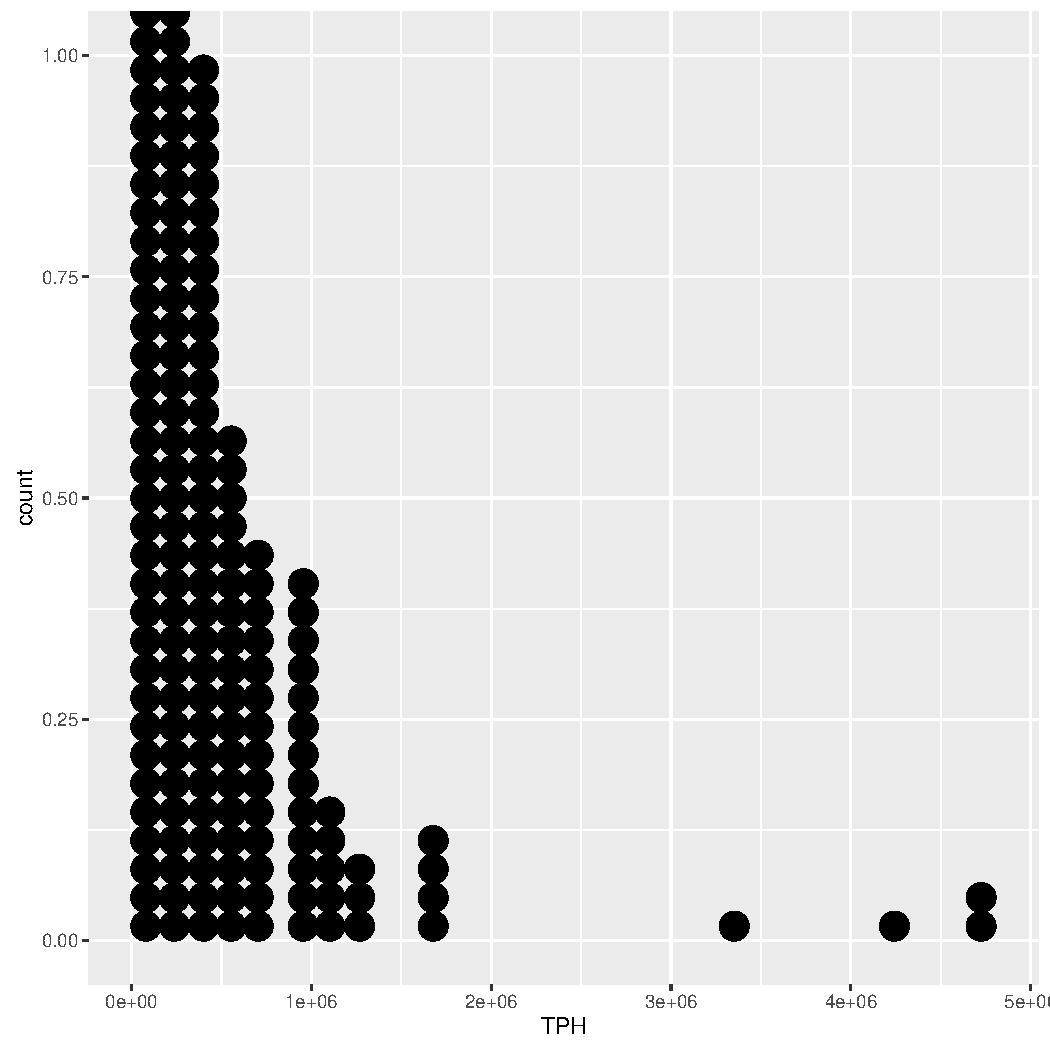
\includegraphics[width=\maxwidth]{figure/atipicos-1} 

\end{knitrout}
	\caption{Dotplot de la variable TPH}
\end{figure}

Con el resultado del gráfico anterior se puede visualizar varios datos atípicos, aunque los datos son consistentes se procede mejor a realizar un análisis del DataSet más detallado, de acuerdo con la información que se tiene de los diferentes años de la muestra.

%\vspace{-10mm}
%\subsection{Analizando población hispana en el año 1990}
%Los datos más representativos se dan a continuación:

% Table created by stargazer v.5.2 by Marek Hlavac, Harvard University. E-mail: hlavac at fas.harvard.edu
% Date and time: vie, may 13, 2016 - 10:06:38 p.m.
\begin{table}[!htbp] \centering 
  \caption{Total de la población de EEUU en el año 1990} 
  \label{} 
\begin{tabular}{@{\extracolsep{5pt}}lccccc} 
\\[-1.8ex]\hline 
\hline \\[-1.8ex] 
Statistic & \multicolumn{1}{c}{N} & \multicolumn{1}{c}{Mean} & \multicolumn{1}{c}{St. Dev.} & \multicolumn{1}{c}{Min} & \multicolumn{1}{c}{Max} \\ 
\hline \\[-1.8ex] 
TP & 3,136 & 79,300.610 & 264,006.100 & 107 & 8,863,164 \\ 
TPNH & 3,136 & 72,172.490 & 208,127.900 & 93 & 5,511,922 \\ 
TPH & 3,136 & 7,128.126 & 71,748.130 & 0 & 3,351,242 \\ 
\hline \\[-1.8ex] 
\end{tabular} 
\end{table} 


%\vspace{-10mm}
%\subsection{Analizando población hispana en el año 2000}
%Los datos más representativos se dan a continuación:

% Table created by stargazer v.5.2 by Marek Hlavac, Harvard University. E-mail: hlavac at fas.harvard.edu
% Date and time: vie, may 13, 2016 - 10:06:38 p.m.
\begin{table}[!htbp] \centering 
  \caption{Total de la población de EEUU en el año 2000} 
  \label{} 
\begin{tabular}{@{\extracolsep{5pt}}lccccc} 
\\[-1.8ex]\hline 
\hline \\[-1.8ex] 
Statistic & \multicolumn{1}{c}{N} & \multicolumn{1}{c}{Mean} & \multicolumn{1}{c}{St. Dev.} & \multicolumn{1}{c}{Min} & \multicolumn{1}{c}{Max} \\ 
\hline \\[-1.8ex] 
TP & 3,136 & 89,735.040 & 292,674.700 & 67 & 9,519,338 \\ 
TPNH & 3,136 & 78,476.900 & 214,891.300 & 60 & 5,277,125 \\ 
TPH & 3,136 & 11,258.140 & 96,312.440 & 1 & 4,242,213 \\ 
\hline \\[-1.8ex] 
\end{tabular} 
\end{table} 


%\vspace{-10mm}
%\subsection{Analizando población hispana en el año 2010}
%Los datos más representativos se dan a continuación:

% Table created by stargazer v.5.2 by Marek Hlavac, Harvard University. E-mail: hlavac at fas.harvard.edu
% Date and time: vie, may 13, 2016 - 10:06:38 p.m.
\begin{table}[!htbp] \centering 
  \caption{Total de la población de EEUU en el año 2010} 
  \label{} 
\begin{tabular}{@{\extracolsep{5pt}}lccccc} 
\\[-1.8ex]\hline 
\hline \\[-1.8ex] 
Statistic & \multicolumn{1}{c}{N} & \multicolumn{1}{c}{Mean} & \multicolumn{1}{c}{St. Dev.} & \multicolumn{1}{c}{Min} & \multicolumn{1}{c}{Max} \\ 
\hline \\[-1.8ex] 
TP & 3,136 & 98,430.440 & 313,221.000 & 82 & 9,818,605 \\ 
TPNH & 3,136 & 82,336.350 & 216,856.000 & 64 & 5,130,716 \\ 
TPH & 3,136 & 16,094.090 & 115,731.900 & 0 & 4,687,889 \\ 
\hline \\[-1.8ex] 
\end{tabular} 
\end{table} 


%\vspace{-10mm}
%\subsection{Analizando población hispana en el año 2011}
%Los datos más representativos se dan a continuación:

% Table created by stargazer v.5.2 by Marek Hlavac, Harvard University. E-mail: hlavac at fas.harvard.edu
% Date and time: vie, may 13, 2016 - 10:06:38 p.m.
\begin{table}[!htbp] \centering 
  \caption{Total de la población de EEUU en el año 2011} 
  \label{} 
\begin{tabular}{@{\extracolsep{5pt}}lccccc} 
\\[-1.8ex]\hline 
\hline \\[-1.8ex] 
Statistic & \multicolumn{1}{c}{N} & \multicolumn{1}{c}{Mean} & \multicolumn{1}{c}{St. Dev.} & \multicolumn{1}{c}{Min} & \multicolumn{1}{c}{Max} \\ 
\hline \\[-1.8ex] 
TP & 3,136 & 99,337.630 & 316,723.400 & 90 & 9,889,056 \\ 
TPNH & 3,136 & 82,743.800 & 217,998.000 & 76 & 5,128,082 \\ 
TPH & 3,136 & 16,593.830 & 118,221.400 & 0 & 4,760,974 \\ 
\hline \\[-1.8ex] 
\end{tabular} 
\end{table} 



%\vspace{-10mm}
\begin{figure}[H]
	\centering
\begin{knitrout}
\definecolor{shadecolor}{rgb}{0.969, 0.969, 0.969}\color{fgcolor}
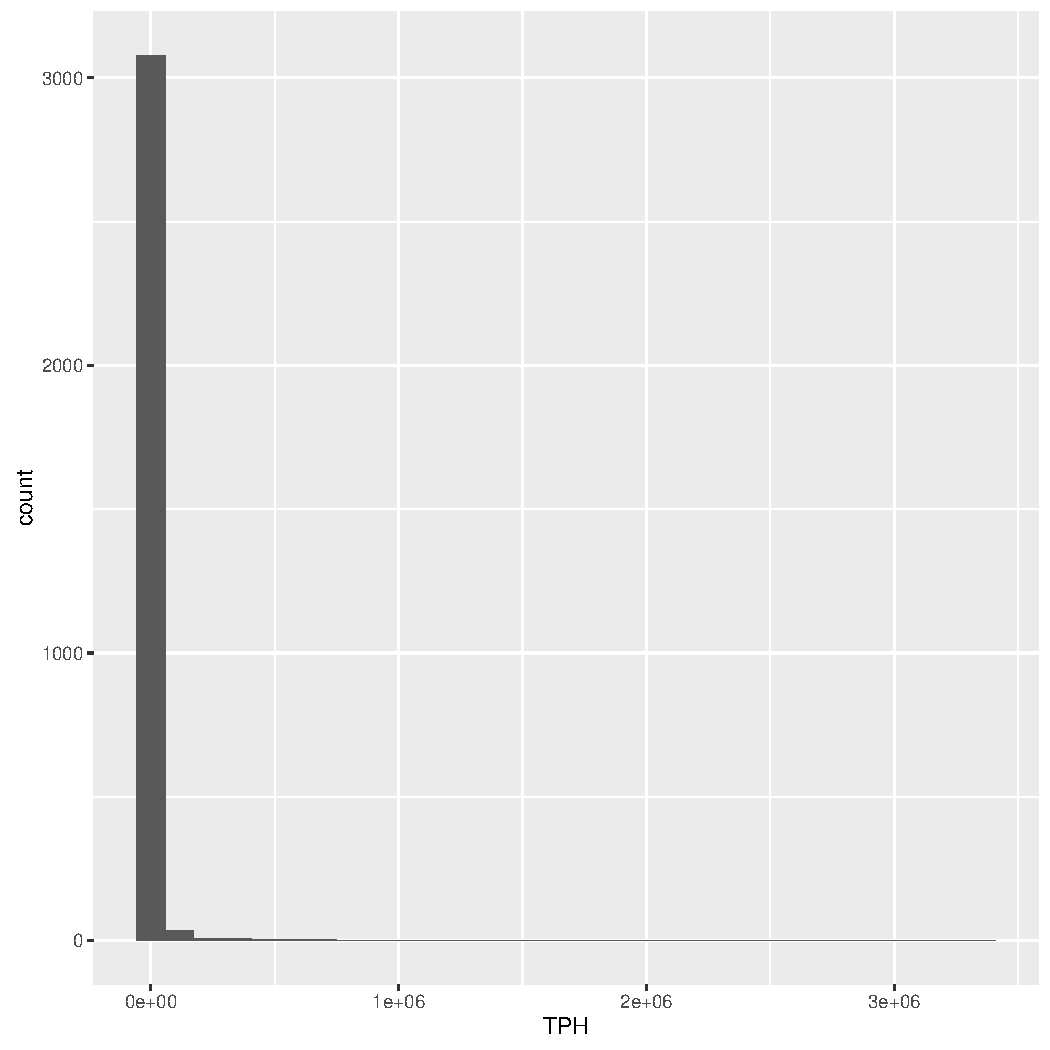
\includegraphics[width=\maxwidth]{figure/pobHis1990-1} 

\end{knitrout}
	\caption{Población Hispana en el año 1990}
\end{figure}


%\vspace{-5mm}
\begin{figure}[H]
	\centering
\begin{knitrout}
\definecolor{shadecolor}{rgb}{0.969, 0.969, 0.969}\color{fgcolor}
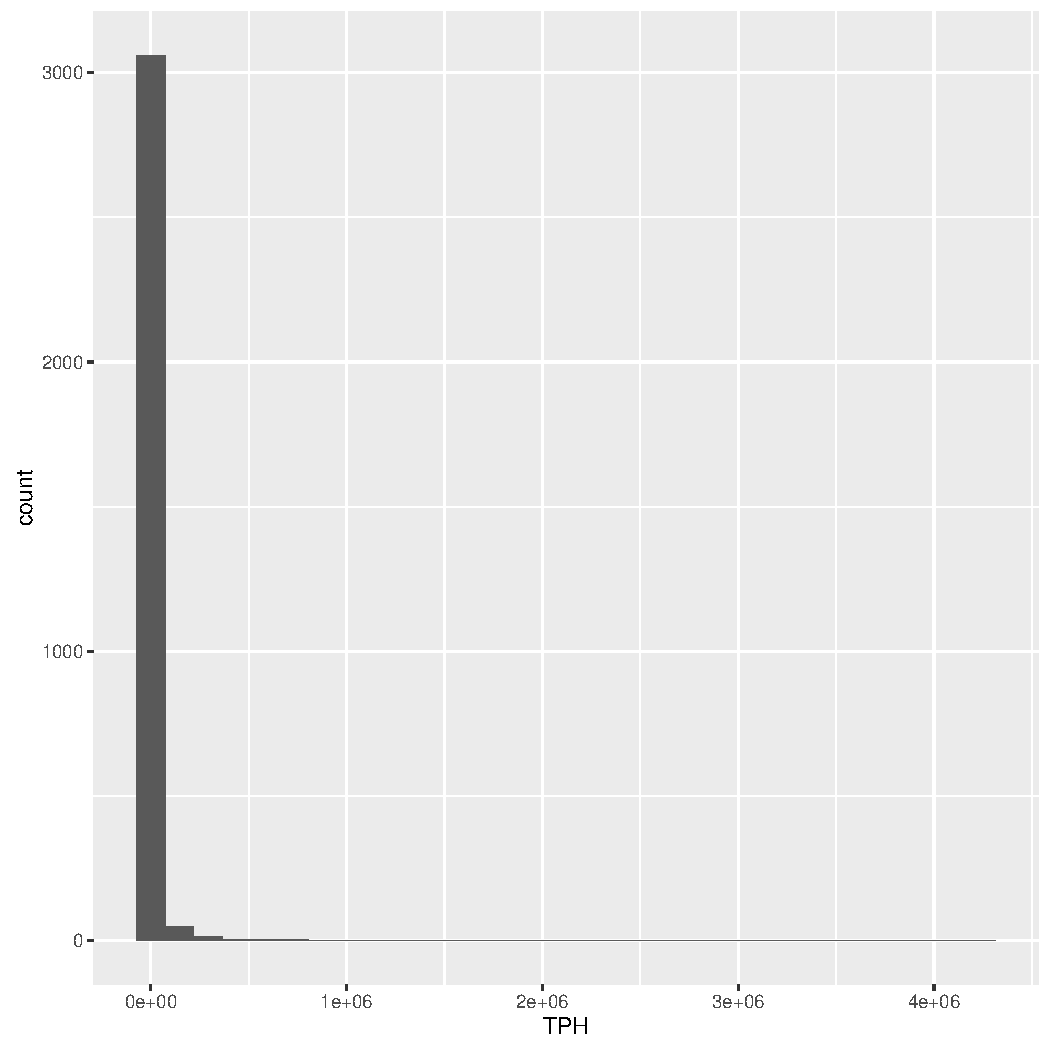
\includegraphics[width=\maxwidth]{figure/pobHisp2000-1} 

\end{knitrout}
	\caption{Población Hispana en el año 2000}
\end{figure}


%\vspace{-5mm}
\begin{figure}[H]
	\centering
\begin{knitrout}
\definecolor{shadecolor}{rgb}{0.969, 0.969, 0.969}\color{fgcolor}
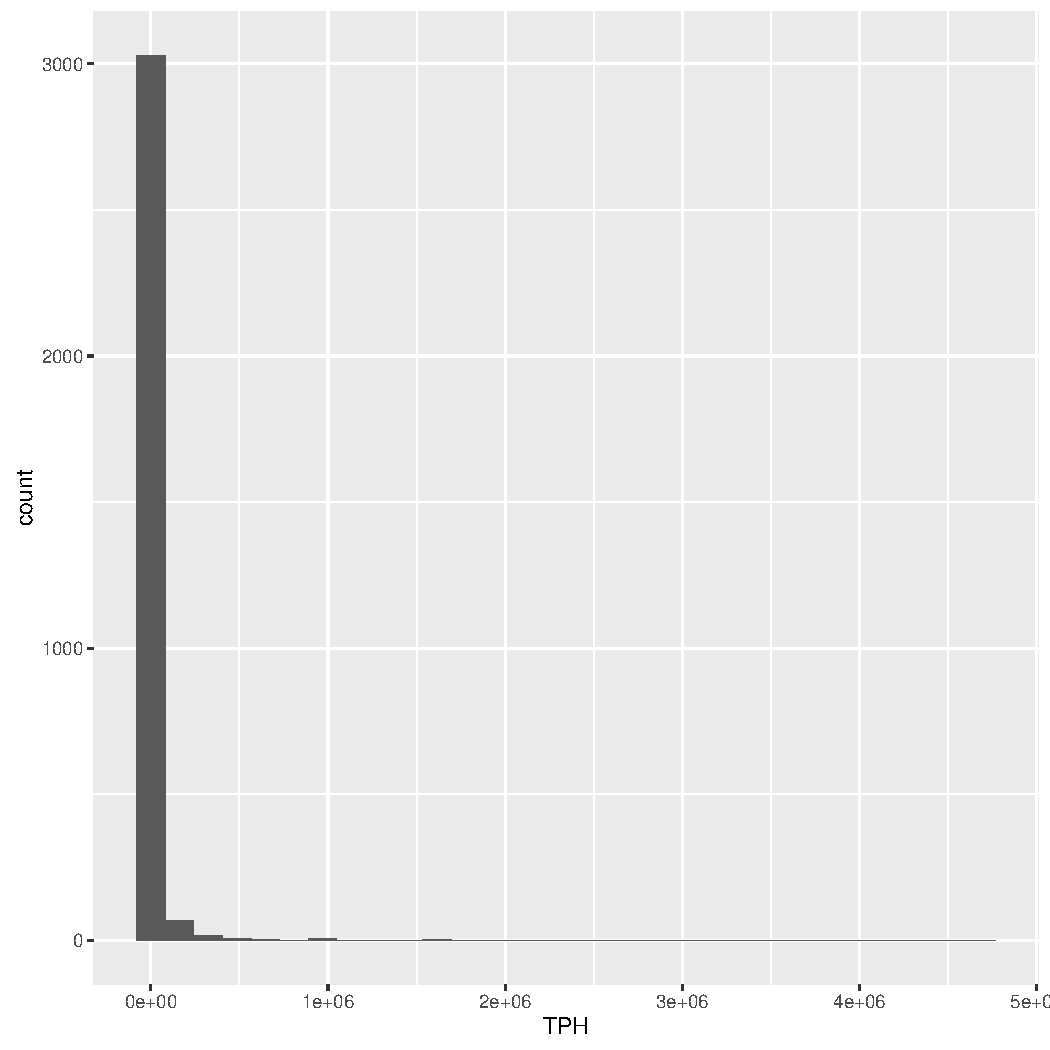
\includegraphics[width=\maxwidth]{figure/pobHisp2010-1} 

\end{knitrout}
	\caption{Población Hispana en el año 2010}
\end{figure}


%\vspace{-10mm}
\begin{figure}[H]
	\centering
\begin{knitrout}
\definecolor{shadecolor}{rgb}{0.969, 0.969, 0.969}\color{fgcolor}
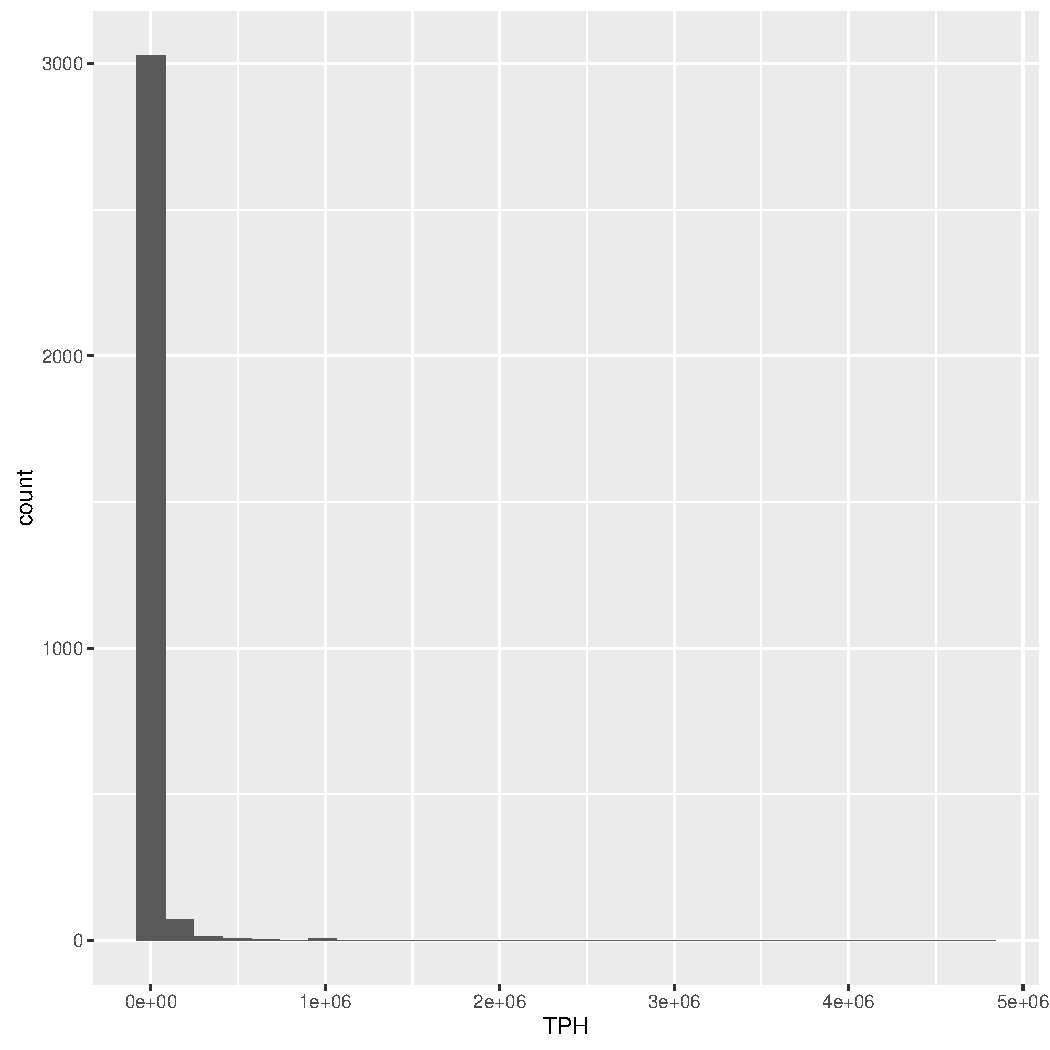
\includegraphics[width=\maxwidth]{figure/pobHisp2011-1} 

\end{knitrout}
	\caption{Población Hispana en el año 2011}
\end{figure}

%\vspace{-10mm}
\subsection{Percentiles del conjunto de datos}
El percentil de orden \(k\) es el cuantil de orden \(\dfrac {k} {100}\). El recorrido intercuantil refleja la variabilidad de las observaciones comprendidas entre los percentiles 25 y 75 en el conjunto de datos. En esta sesión se obtienen los percentiles del 25\%,  50\% y 75\% de las variables Total Población (TP) y Total Población Hispana (TPH) en los diferentes años de la muestra.

%\vspace{4mm}
%\begin{itemize}
%\item Percentiles del población en el año 1990
% latex table generated in R 3.2.3 by xtable 1.8-2 package
% Fri May 13 22:06:39 2016
\begin{table}[ht]
\centering
\begin{tabular}{rrrr}
  \hline
 & PercentilesTP & PercentilesTPH & PercentilesTPNH \\ 
  \hline
25\% & 10360.00 & 67.00 & 9836.75 \\ 
  50\% & 22224.00 & 208.00 & 21362.00 \\ 
  75\% & 54771.50 & 1159.00 & 53324.00 \\ 
   \hline
\end{tabular}
\caption{Percentiles de TP, TPH y TPNH en el año 1990} 
\end{table}


% latex table generated in R 3.2.3 by xtable 1.8-2 package
% Fri May 13 22:06:39 2016
\begin{table}[ht]
\centering
\begin{tabular}{rrrr}
  \hline
 & PercentilesTP & PercentilesTPH & PercentilesTPNH \\ 
  \hline
25\% & 11264.25 & 155.00 & 10431.50 \\ 
  50\% & 24658.00 & 493.00 & 23244.00 \\ 
  75\% & 61844.25 & 2411.50 & 58906.00 \\ 
   \hline
\end{tabular}
\caption{Percentiles de TP, TPH y TPNH en el año 2000} 
\end{table}

	
% latex table generated in R 3.2.3 by xtable 1.8-2 package
% Fri May 13 22:06:39 2016
\begin{table}[ht]
\centering
\begin{tabular}{rrrr}
  \hline
 & PercentilesTP & PercentilesTPH & PercentilesTPNH \\ 
  \hline
25\% & 11154.75 & 262.75 & 10154.25 \\ 
  50\% & 25901.50 & 892.00 & 24016.00 \\ 
  75\% & 67012.50 & 4226.25 & 62438.50 \\ 
   \hline
\end{tabular}
\caption{Percentiles de TP, TPH y TPNH en el año 2010} 
\end{table}

	
% latex table generated in R 3.2.3 by xtable 1.8-2 package
% Fri May 13 22:06:39 2016
\begin{table}[ht]
\centering
\begin{tabular}{rrrr}
  \hline
 & PercentilesTP & PercentilesTPH & PercentilesTPNH \\ 
  \hline
25\% & 11145.00 & 284.00 & 10125.75 \\ 
  50\% & 25896.00 & 926.00 & 23962.00 \\ 
  75\% & 67398.75 & 4417.75 & 62925.75 \\ 
   \hline
\end{tabular}
\caption{Percentiles de TP, TPH y TPNH en el año 2011} 
\end{table}

	
	% Solución de preguntas

\section{Solución de Preguntas}
Ahora se procederá a responder todas las preguntas que se plantearón al inicio de la investigación.



\subsection{Caracter descriptivo}

%\begin{enumerate}
%A continuación se enumeran los promedios de la variable total ploblación en cada uno de los años del DataSet:
%\item los promedios por  año de los ciudadanos en EEUU, son los siguientes\\
%\begin{itemize}
%\item promedio del año 1990:
%<<unoa, results='asis', echo=FALSE, warning=FALSE, message=FALSE>>=
%	mean(datos1990$TP)
%@
%\item promedio del año 2000:
%<<unob,results='asis',echo=FALSE, warning=FALSE, message=FALSE>>=
%	mean(datos2000$TP)
%@
%\item promedio del año 2010:
%<<unoc,results='asis',echo=FALSE, warning=FALSE, message=FALSE>>=
%	mean(datos2010$TP)
%@
%\item promedio del año 2011:
%<<unod, results='asis', echo=FALSE, warning=FALSE, message=FALSE>>=
%	mean(datos2011$TP)
%@
%\end{itemize}

A continuación se enumeran las medias de la variables Total Población (TP), Total Población  No Hispana (TPNH) y Total Ploblación Hispana (TPH) en cada uno de los años del DataSet:

% latex table generated in R 3.2.3 by xtable 1.8-2 package
% Fri May 13 22:06:39 2016
\begin{table}[ht]
\centering
\begin{tabular}{rrrrr}
  \hline
 & Año 1990 & Año 2000 & Año 2010 & Año 2011 \\ 
  \hline
Media TP & 79300.61 & 89735.04 & 98430.44 & 99337.63 \\ 
  Media TPNH & 72172.49 & 78476.90 & 82336.35 & 82743.80 \\ 
  Media TPH & 7128.13 & 11258.14 & 16094.09 & 16593.83 \\ 
   \hline
\end{tabular}
\caption{Valores de las medias en TP, TPHN y TPH} 
\end{table}


%\item Ciudad con más población en 1990
% latex table generated in R 3.2.3 by xtable 1.8-2 package
% Fri May 13 22:06:39 2016
\begin{table}[ht]
\centering
\begin{tabular}{rllr}
  \hline
 & Ciudad & Estado & Poblacion \\ 
  \hline
1 & Los Angeles & California & 8863164 \\ 
   \hline
\end{tabular}
\caption{Ciudad con más población en el año 1990} 
\end{table}


%Ciudades con menos población en el año 1990
% latex table generated in R 3.2.3 by xtable 1.8-2 package
% Fri May 13 22:06:39 2016
\begin{table}[ht]
\centering
\begin{tabular}{rllr}
  \hline
 & Ciudad & Estado & Poblacion \\ 
  \hline
1 & Loving & Texas & 107 \\ 
   \hline
\end{tabular}
\caption{Ciudad con menos población en el año 1990} 
\end{table}


%\item Ciudad con más población en 2000
% latex table generated in R 3.2.3 by xtable 1.8-2 package
% Fri May 13 22:06:39 2016
\begin{table}[ht]
\centering
\begin{tabular}{rllr}
  \hline
 & Ciudad & Estado & Poblacion \\ 
  \hline
1 & Los Angeles & California & 8863164 \\ 
   \hline
\end{tabular}
\caption{Ciudad con más población en el año 2000} 
\end{table}


%Ciudades con menos población en el año 2000
% latex table generated in R 3.2.3 by xtable 1.8-2 package
% Fri May 13 22:06:39 2016
\begin{table}[ht]
\centering
\begin{tabular}{rllr}
  \hline
 & Ciudad & Estado & Poblacion \\ 
  \hline
1 & Loving & Texas &  67 \\ 
   \hline
\end{tabular}
\caption{Ciudad con menos población en el año 2000} 
\end{table}


%\item Ciudad con más población en 2010
% latex table generated in R 3.2.3 by xtable 1.8-2 package
% Fri May 13 22:06:39 2016
\begin{table}[ht]
\centering
\begin{tabular}{rllr}
  \hline
 & Ciudad & Estado & Poblacion \\ 
  \hline
1 & Los Angeles & California & 9818605 \\ 
   \hline
\end{tabular}
\caption{Ciudad con más población en el año 2010} 
\end{table}


%Ciudades con menos población en el año 2010
% latex table generated in R 3.2.3 by xtable 1.8-2 package
% Fri May 13 22:06:39 2016
\begin{table}[ht]
\centering
\begin{tabular}{rllr}
  \hline
 & Ciudad & Estado & Poblacion \\ 
  \hline
1 & Loving & Texas &  82 \\ 
   \hline
\end{tabular}
\caption{Ciudad con menos pobl. en 2010} 
\end{table}


%\item Ciudad con más población en 2011
% latex table generated in R 3.2.3 by xtable 1.8-2 package
% Fri May 13 22:06:40 2016
\begin{table}[ht]
\centering
\begin{tabular}{rllr}
  \hline
 & Ciudad & Estado & Poblacion \\ 
  \hline
1 & Los Angeles & California & 9889056 \\ 
   \hline
\end{tabular}
\caption{Ciudad con más población en el año 2011} 
\end{table}


%Ciudades con menos población en el año 2011
% latex table generated in R 3.2.3 by xtable 1.8-2 package
% Fri May 13 22:06:40 2016
\begin{table}[ht]
\centering
\begin{tabular}{rllr}
  \hline
 & Ciudad & Estado & Poblacion \\ 
  \hline
1 & Kalawao & Hawaii &  90 \\ 
   \hline
\end{tabular}
\caption{Ciudad con menos población en el año 2011} 
\end{table}


%A continuación se enumera las medias de la variables Total Población (TP), Total Población  No Hispana (TPNH) y Total Ploblación Hispana (TPH) en cada uno de los años del DataSet:
%\item los promedios por año de ciudadanos hispanos, son los siguientes\\
%\begin{itemize}
%\item promedio del año 1990:
%<<mseisa,results='asis',echo=FALSE, warning=FALSE, message=FALSE>>=
%	mean(datos1990$TPH)
%@
%\item promedio del año 2000:
%<<seisb,results='asis',echo=FALSE, warning=FALSE, message=FALSE>>=
%	mean(datos2000$TPH)
%@
%\item promedio del año 2010:
%<<seisc,results='asis',echo=FALSE, warning=FALSE, message=FALSE>>=
%	mean(datos2010$TPH)
%@
%\item promedio del año 2011:
%<<seisd,results='asis',echo=FALSE, warning=FALSE, message=FALSE>>=
%	mean(datos2011$TPH)
%@
%\end{itemize}
%	grupoMediaTP 	<- c(mean(datos1990$TP), mean(datos2000$TP), mean(datos2010$TP), mean(datos2011$TP))
%	grupoMediaTPNH 	<- c(mean(datos1990$TPNH), mean(datos2000$TPNH), mean(datos2010$TPNH),  mean(datos2011$TPNH))
%	grupoMediaTPH 	<- c(mean(datos1990$TPH), mean(datos2000$TPH), mean(datos2010$TPH), mean(datos2011$TPH))
%	mediasFull<-data.frame(TP=grupoMediaTP, TPNH=grupoMediaTPNH, TPH=grupoMediaTPH)	 	
%	xtable(mediasFull,"Valores de las medias en TP, TPHN y TPH")

El análisis continua con los siguientes resultados.
%Ciudad con mas población hispana en el año 1990
% latex table generated in R 3.2.3 by xtable 1.8-2 package
% Fri May 13 22:06:40 2016
\begin{table}[ht]
\centering
\begin{tabular}{rllr}
  \hline
 & Ciudad & Estado & PoblacionH \\ 
  \hline
1 & Los Angeles & California & 3351242 \\ 
   \hline
\end{tabular}
\caption{Ciudad con mayor TPH en el año 1990} 
\end{table}


%Ciudades con menos población hispana en el año 1990
% latex table generated in R 3.2.3 by xtable 1.8-2 package
% Fri May 13 22:06:40 2016
\begin{table}[ht]
\centering
\begin{tabular}{rllr}
  \hline
 & Ciudad & Estado & PoblacionH \\ 
  \hline
1 & Garfield & Montana &   0 \\ 
  2 & Petroleum & Montana &   0 \\ 
  3 & Arthur & Nebraska &   0 \\ 
  4 & Blaine & Nebraska &   0 \\ 
  5 & McPherson & Nebraska &   0 \\ 
  6 & Wheeler & Nebraska &   0 \\ 
  7 & Billings & North Dakota &   0 \\ 
  8 & Campbell & South Dakota &   0 \\ 
  9 & McPherson & South Dakota &   0 \\ 
   \hline
\end{tabular}
\caption{Ciudad con menor TPH en el año 1990} 
\end{table}


%Ciudad con más población hispana en el año 2000
% latex table generated in R 3.2.3 by xtable 1.8-2 package
% Fri May 13 22:06:40 2016
\begin{table}[ht]
\centering
\begin{tabular}{rllr}
  \hline
 & Ciudad & Estado & PoblacionH \\ 
  \hline
1 & Los Angeles & California & 4242213 \\ 
   \hline
\end{tabular}
\caption{Ciudad con mayor TPH en el año 2000} 
\end{table}


%Ciudades con menos población hispana en el año 2000
% latex table generated in R 3.2.3 by xtable 1.8-2 package
% Fri May 13 22:06:40 2016
\begin{table}[ht]
\centering
\begin{tabular}{rllr}
  \hline
 & Ciudad & Estado & PoblacionH \\ 
  \hline
1 & Blaine & Nebraska &   1 \\ 
  2 & Slope & North Dakota &   1 \\ 
   \hline
\end{tabular}
\caption{Ciudad con menor TPH en el año 2000} 
\end{table}


%Ciudad con más población hispana en el año 2010
% latex table generated in R 3.2.3 by xtable 1.8-2 package
% Fri May 13 22:06:40 2016
\begin{table}[ht]
\centering
\begin{tabular}{rllr}
  \hline
 & Ciudad & Estado & PoblacionH \\ 
  \hline
1 & Los Angeles & California & 4687889 \\ 
   \hline
\end{tabular}
\caption{Ciudad con mayor TPH en el año 2010} 
\end{table}


%Ciudad con menos población hispana en el año 2010
% latex table generated in R 3.2.3 by xtable 1.8-2 package
% Fri May 13 22:06:40 2016
\begin{table}[ht]
\centering
\begin{tabular}{rllr}
  \hline
 & Ciudad & Estado & PoblacionH \\ 
  \hline
1 & Blaine & Nebraska &   0 \\ 
   \hline
\end{tabular}
\caption{Ciudad con menor TPH en el año 2010} 
\end{table}


%Ciudad con más población hispana en el año 2011
% latex table generated in R 3.2.3 by xtable 1.8-2 package
% Fri May 13 22:06:40 2016
\begin{table}[ht]
\centering
\begin{tabular}{rllr}
  \hline
 & Ciudad & Estado & PoblacionH \\ 
  \hline
1 & Los Angeles & California & 4760974 \\ 
   \hline
\end{tabular}
\caption{Ciudad con mayor TPH en el año 2011} 
\end{table}


%Ciudad con menos población hispana en el año 2011
% latex table generated in R 3.2.3 by xtable 1.8-2 package
% Fri May 13 22:06:40 2016
\begin{table}[ht]
\centering
\begin{tabular}{rllr}
  \hline
 & Ciudad & Estado & PoblacionH \\ 
  \hline
1 & Blaine & Nebraska &   0 \\ 
   \hline
\end{tabular}
\caption{Ciudad con menor TPH en el año 2011} 
\end{table}


\subsection{Matriz de correlación}
A continuación se visualiza la matriz de correlación que existe entre la variables cuantitativas del conjunto de datos: 
%Ciudad con menos población hispana en el año 2011
% latex table generated in R 3.2.3 by xtable 1.8-2 package
% Fri May 13 22:06:40 2016
\begin{table}[ht]
\centering
\begin{tabular}{rrrrrr}
  \hline
 & TP & TPNH & TPH & PPH & AP \\ 
  \hline
TP & 1.00 & 0.97 & 0.87 & 0.17 & 0.03 \\ 
  TPNH & 0.97 & 1.00 & 0.73 & 0.12 & 0.02 \\ 
  TPH & 0.87 & 0.73 & 1.00 & 0.25 & 0.04 \\ 
  PPH & 0.17 & 0.12 & 0.25 & 1.00 & 0.13 \\ 
  AP & 0.03 & 0.02 & 0.04 & 0.13 & 1.00 \\ 
   \hline
\end{tabular}
\caption{Matrix de correlación} 
\end{table}

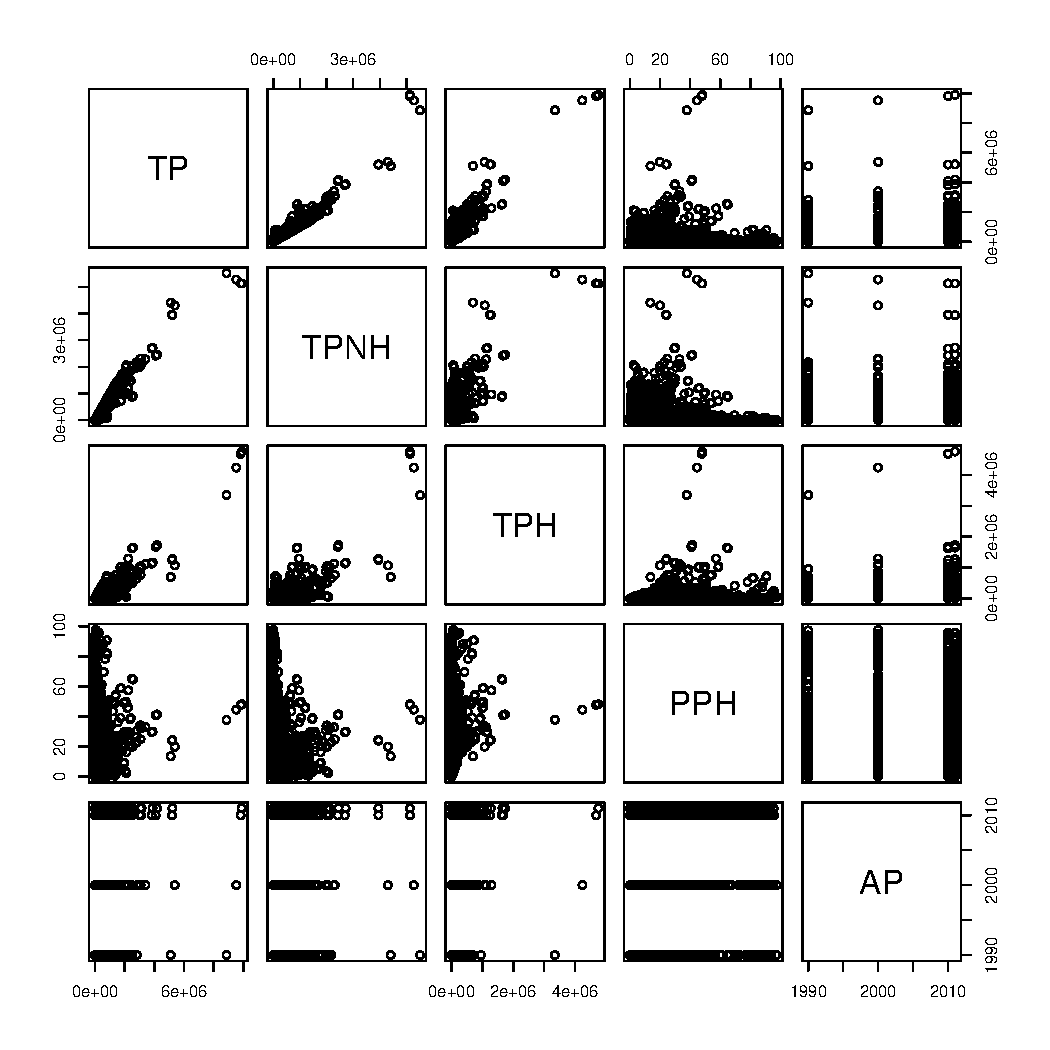
\includegraphics[width=\maxwidth]{figure/correlacion-1} 

	
	%BIBLIOGRAFÍA
	%ENTORNO {thebibliography}
	%Permite al autor listar las referencias utilizadas y citarlas en algun punto del texto.
	
	\newpage
	 \begin{thebibliography}{1}
	 	
	 	\bibitem{biblio1}
	 	S. Mohanty, M. Jagadeesh and H. Srivatsa, Big Data Imperatives: Enterprise Big Data Warehouse, BI Implementations and Analytics, Published Apress, Isbn: 978-1-4302-4872-9, New York, 2013.
	 	
	 	\bibitem{biblio2}
	 	pewhispanic.org, Pew Research Center’s Hispanic Trends Project, U.S. Hispanic Population by County, 1980-2011. Disponible en: http://www.pewhispanic.org/2013/08/29/u-s-hispanic-population-by-county-1980-2011/, 2013.
	 	 	
	 	\bibitem{biblio3}
	 	G. T. Doran, There's a S.M.A.R.T. Way to Write Management's Goals and Objectives, Management Review, Vol. 70, Issue 11, pp. 35-36, 1981.
	 	
	 	\bibitem{biblio4}
	 	R. D. Peng and E. Matsui, The Art of Data Science: A guide for anyone who works whit data, Published Leanpub, Disponible en:http://leanpub.com/artofdatascience, 2015.
	 	 	
	 	\bibitem{biblio5}
	 	Alzate Marco, 250 Conceptos de Probabilidad, variables aleatorias y procesos estocásticos en redes de comunicaciones, Universidad Distrital Fransisco José de Caldas, pag 15-123, 2005.
	 	
 		\bibitem{biblio6}
 		G. C. Canavos, Probabilidad y estadística: Aplicaciones y métodos, Virginia Commonwealth University, Published McGRAW HILL, 1988.
	 	
	 \end{thebibliography}
	
\end{document}
